\documentclass[12pt,a4paper]{article}
\usepackage[utf8]{inputenc}
\usepackage[T1]{fontenc}
\usepackage{amsmath}
\usepackage{textcomp}

\usepackage{geometry}
\geometry{a4paper,left=25mm,right=25mm, top=2cm, bottom=2cm} 

\usepackage{graphicx} %fuer bilder

\usepackage{verbatim}


\usepackage{pgfplots}

 \usepackage{mathptmx}
 \usepackage[scaled=.90]{helvet}
 \usepackage{courier}



\usepackage{listings}
\usepackage{color}

\usepackage{float}
 
\definecolor{dkgreen}{rgb}{0,0.6,0}
\definecolor{gray}{rgb}{0.5,0.5,0.5}
\definecolor{mauve}{rgb}{0.58,0,0.82}

\pagestyle{empty}
\lstset{numbers=left,language=C++}
\lstset{showstringspaces=false,
basicstyle=\ttfamily\footnotesize,
breaklines=true,
tabsize=3,
commentstyle=\color{dkgreen},      % comment style
inputencoding={ansinew},
title=\lstname %zeigt titel der datei an
}

\usepackage{pdfpages} % fuer pdfs
\usepackage{hyperref} % fuer url

%\usepackage{filecontents}
%\begin{filecontents*}{data.csv}
%1,15
%10,52.3
%50,72.8
%100,78.4
%500,87.7
%1000,90.1
%5000,95
%10000,95.2
%100000,95.2
%1000000,95.2
%\end{filecontents*}


%keine einrückungen bei absatz
\parindent 0pt

\begin{document}
\title{Übung 06}
\author{Reinhard Penn, Bernhard Selymes}
\date{April 2015}

\normalsize

%Beginn des Dokuments

\newcommand{\Uebung}{Random}
\newcommand{\srcpath}{../../src}
\newcommand{\simpath}{../../sim}

%Angabe
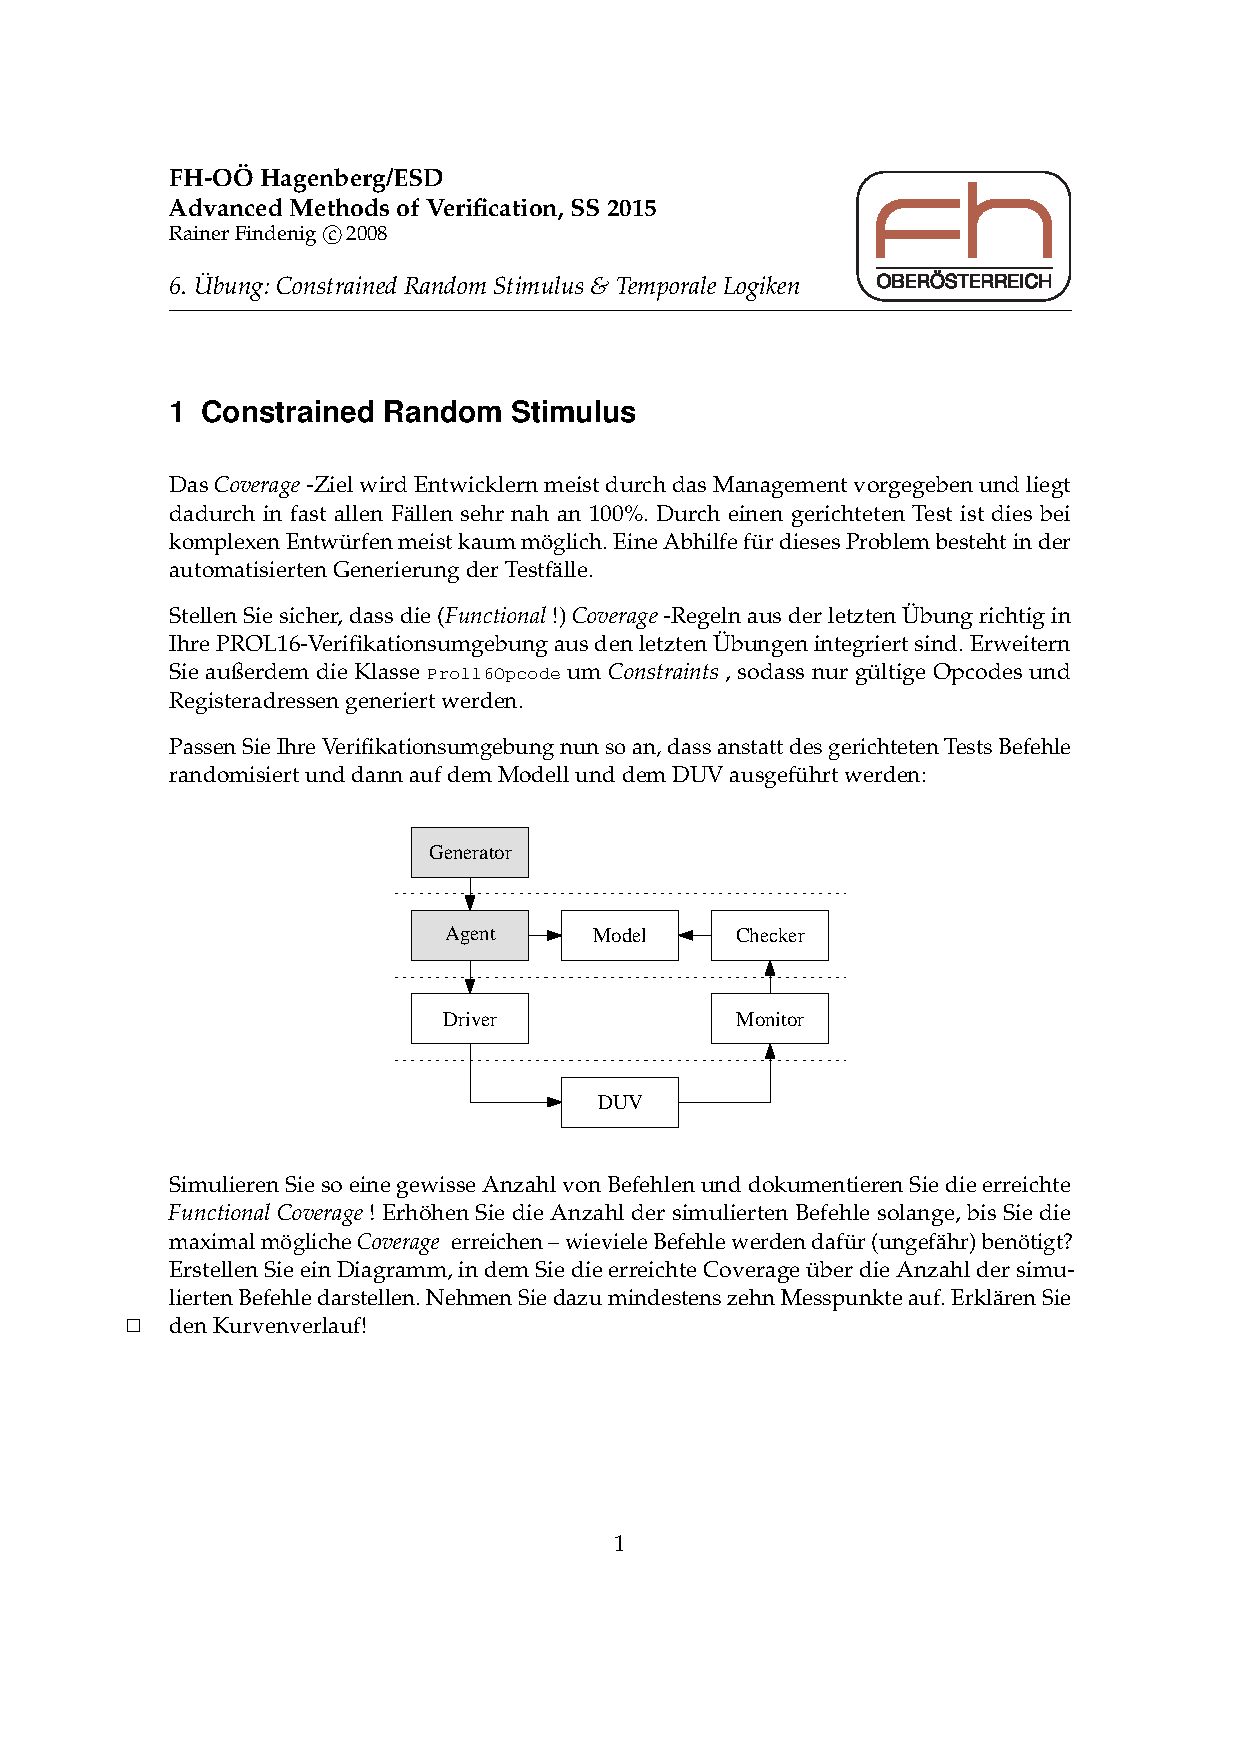
\includepdf[pages=-]{../Angabe.pdf}

\section{Beispiel 1}

\subsection{Diagramm}

\begin{table}[H]
\centering
\begin{tabular}{|l|l|}
\hline
Anzahl  & Coverage (\%) \\ \hline
1       & 15   \\ \hline
10      & 52.3 \\ \hline
50      & 72.8 \\ \hline
100     & 78.4 \\ \hline
500     & 87.7 \\ \hline
1000    & 90.1 \\ \hline
5000    & 95   \\ \hline
10000   & 95.2 \\ \hline
100000  & 95.2 \\ \hline
1000000 & 95.2 \\ \hline
\end{tabular}
\caption{Coverage Tabelle}
\end{table}

\begin{figure}[ht!]
\centering
	\begin{tikzpicture}
		\begin{axis}[xlabel=Anzahl Testfälle, ylabel=Coverage in \%, xmode=log, width=\textwidth]
			\addplot table[col sep=comma, mark=none] {TestabdeckungWerte.csv};
		\end{axis}
	\end{tikzpicture}
	\caption{Coverage Graph \label{overflow}}
\end{figure}

\subsection{Beantwortung der Fragen}

\begin{itemize}
	\item Randomisierte Werte sind vorhersehbar, weil der Randomgenerator einen Seed hat. Die Testfälle sind dadurch reproduzierbar.
	\item Logarithmische Funktion. Je mehr Kombinationen ausgeführt werden desto geringer ist die Chance, dass eine Kombinationen ausgeführt wird, die noch nicht ausgeführt wurde bzw. sind ab einem bestimmten Zeitpunkt alle möglichen Kombinationen ausgeführt worden.
	\item
				\begin{lstlisting}[numbers=none]
constraint ra_0 {
	ra dist { [0:0]:/50, [1:31]:/50 };
}
	
constraint rb_0 {
	rb dist { [0:0]:/50, [1:31]:/50 };
}

constraint nop_0 {
	(cmd == Nop) -> (ra == 0) && (rb == 0);
}
				\end{lstlisting}
		
	\item \texttt{randc} wiederholt Werte erst dann wenn alle ausgeschöpft wurden.
	\item Befehle: 21\\
				Befehle, die keine Flags beeinflussen: 6\\
				Befehle, die beide Flags beeinflussen: 11\\
				Befehle, Carry Flag 0 und Z Flag beeinflussen: 4\\
				
				Berechnung:\\
				keine Flags: 6 * 4 = 24 \\
				Flags: 11 * 4 * 4 = 176 \\
				Carry Flag 0: 4 * 4 * 2 = 32 \\
				Summe: 232 \\
				
				Test aus der Übung: Der Test braucht ca. 5000 Kombinationen, dann ist die maximale Coverage erreicht. Die Redundanz tritt auf, da mehrere Register verwendet werden und dadurch sehr spezielle Kombinationen von Befehlen ausgeführt werden müssen um alle Tests zu covern. Zum Beispiel müssen für ein ADDC sehr spezielle Werte vorhanden sein, damit dieser das Zero und Carry Flag setzt.
				
				
\end{itemize}

\newpage
\subsection{Source Code}

Der Sourcecode des Prol16 wurde nicht hinzugefügt, da der von der Elearning Plattform verwendet wurde.

\lstinputlisting[language={verilog}]{\srcpath/sv/ifProl16.sv}
\lstinputlisting[language={verilog}]{\srcpath/sv/pkgProl16.sv}
\lstinputlisting[language={verilog}]{\srcpath/sv/Prol16Command.sv}
\lstinputlisting[language={verilog}]{\srcpath/sv/Prol16Opcode.sv}
\lstinputlisting[language={verilog}]{\srcpath/sv/Prol16State.sv}
\lstinputlisting[language={verilog}]{\srcpath/sv/Prol16Model.sv}
%\lstinputlisting[language={verilog}]{\srcpath/sv/testProl16Model.sv}
\lstinputlisting[language={verilog}]{\srcpath/sv/testProl16Rand.sv}
\lstinputlisting[language={verilog}]{\srcpath/sv/top.sv}

\lstinputlisting[language={tcl}]{\simpath/CompileSimRandCov.do}

\newpage
\section{Beispiel 2}

\begin{figure}[ht!]
\centering
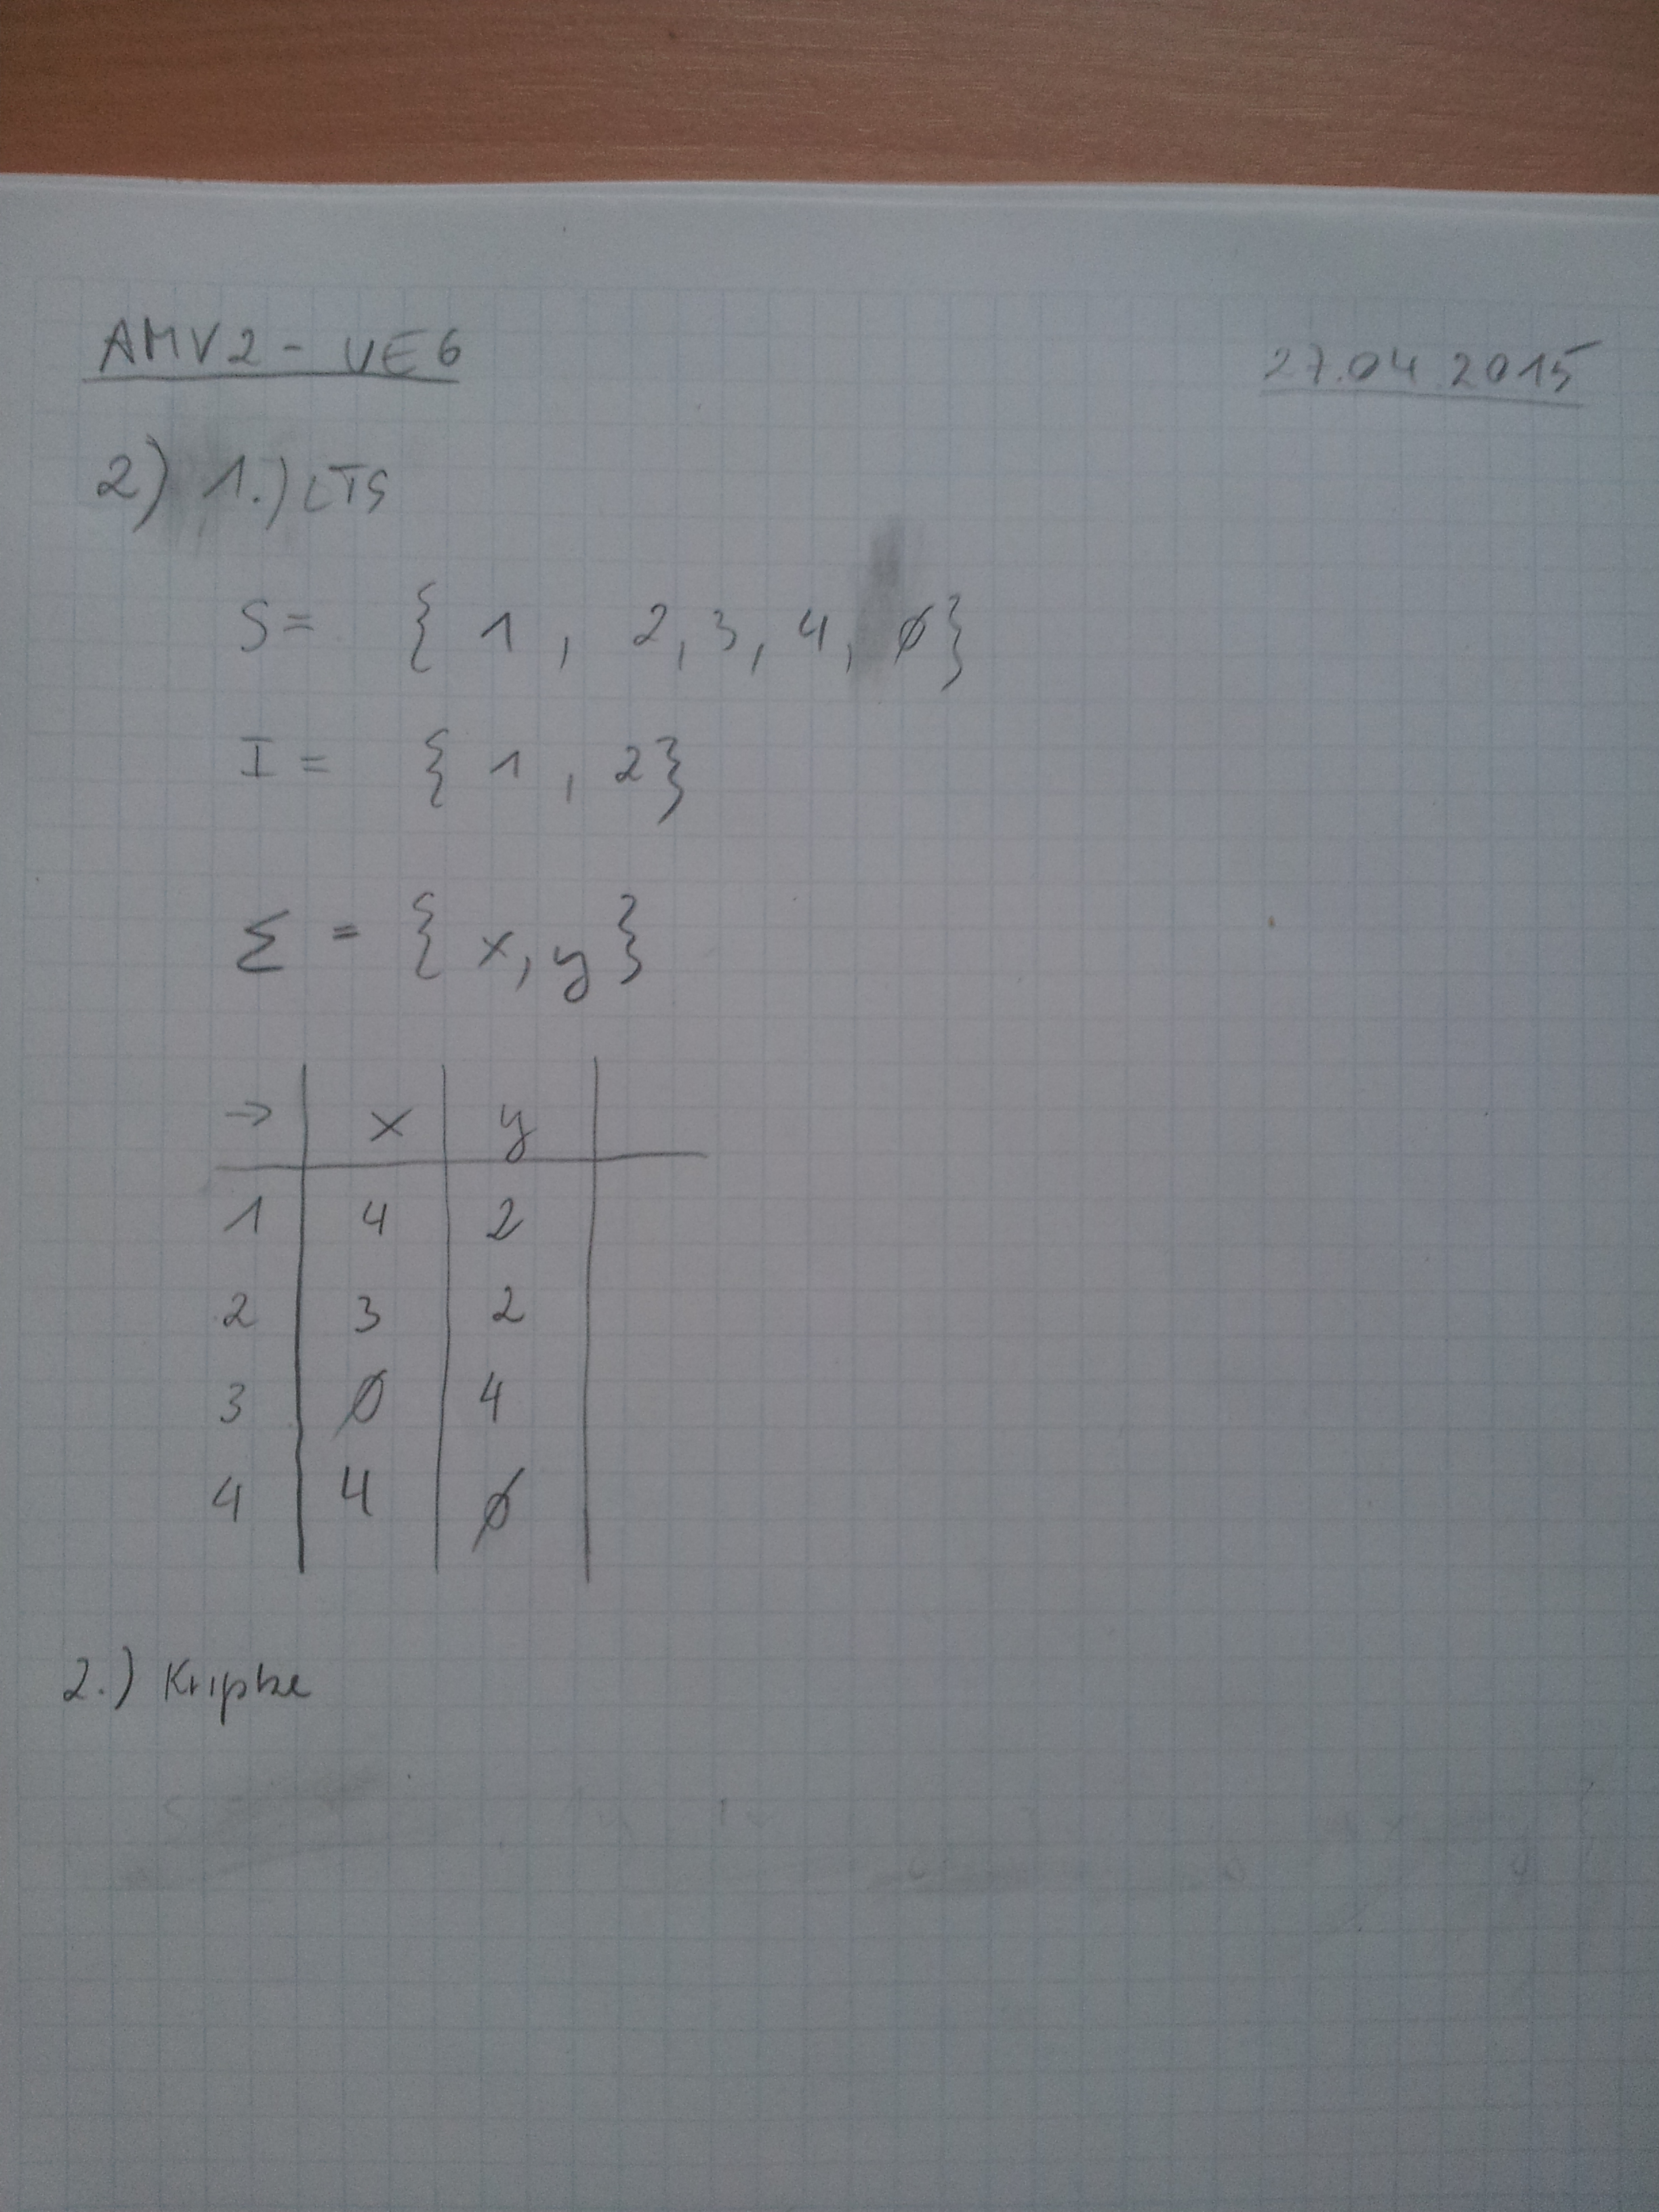
\includegraphics[width=\textwidth]{1.jpg}
\caption{LTS}
\end{figure}

\begin{figure}[ht!]
\centering
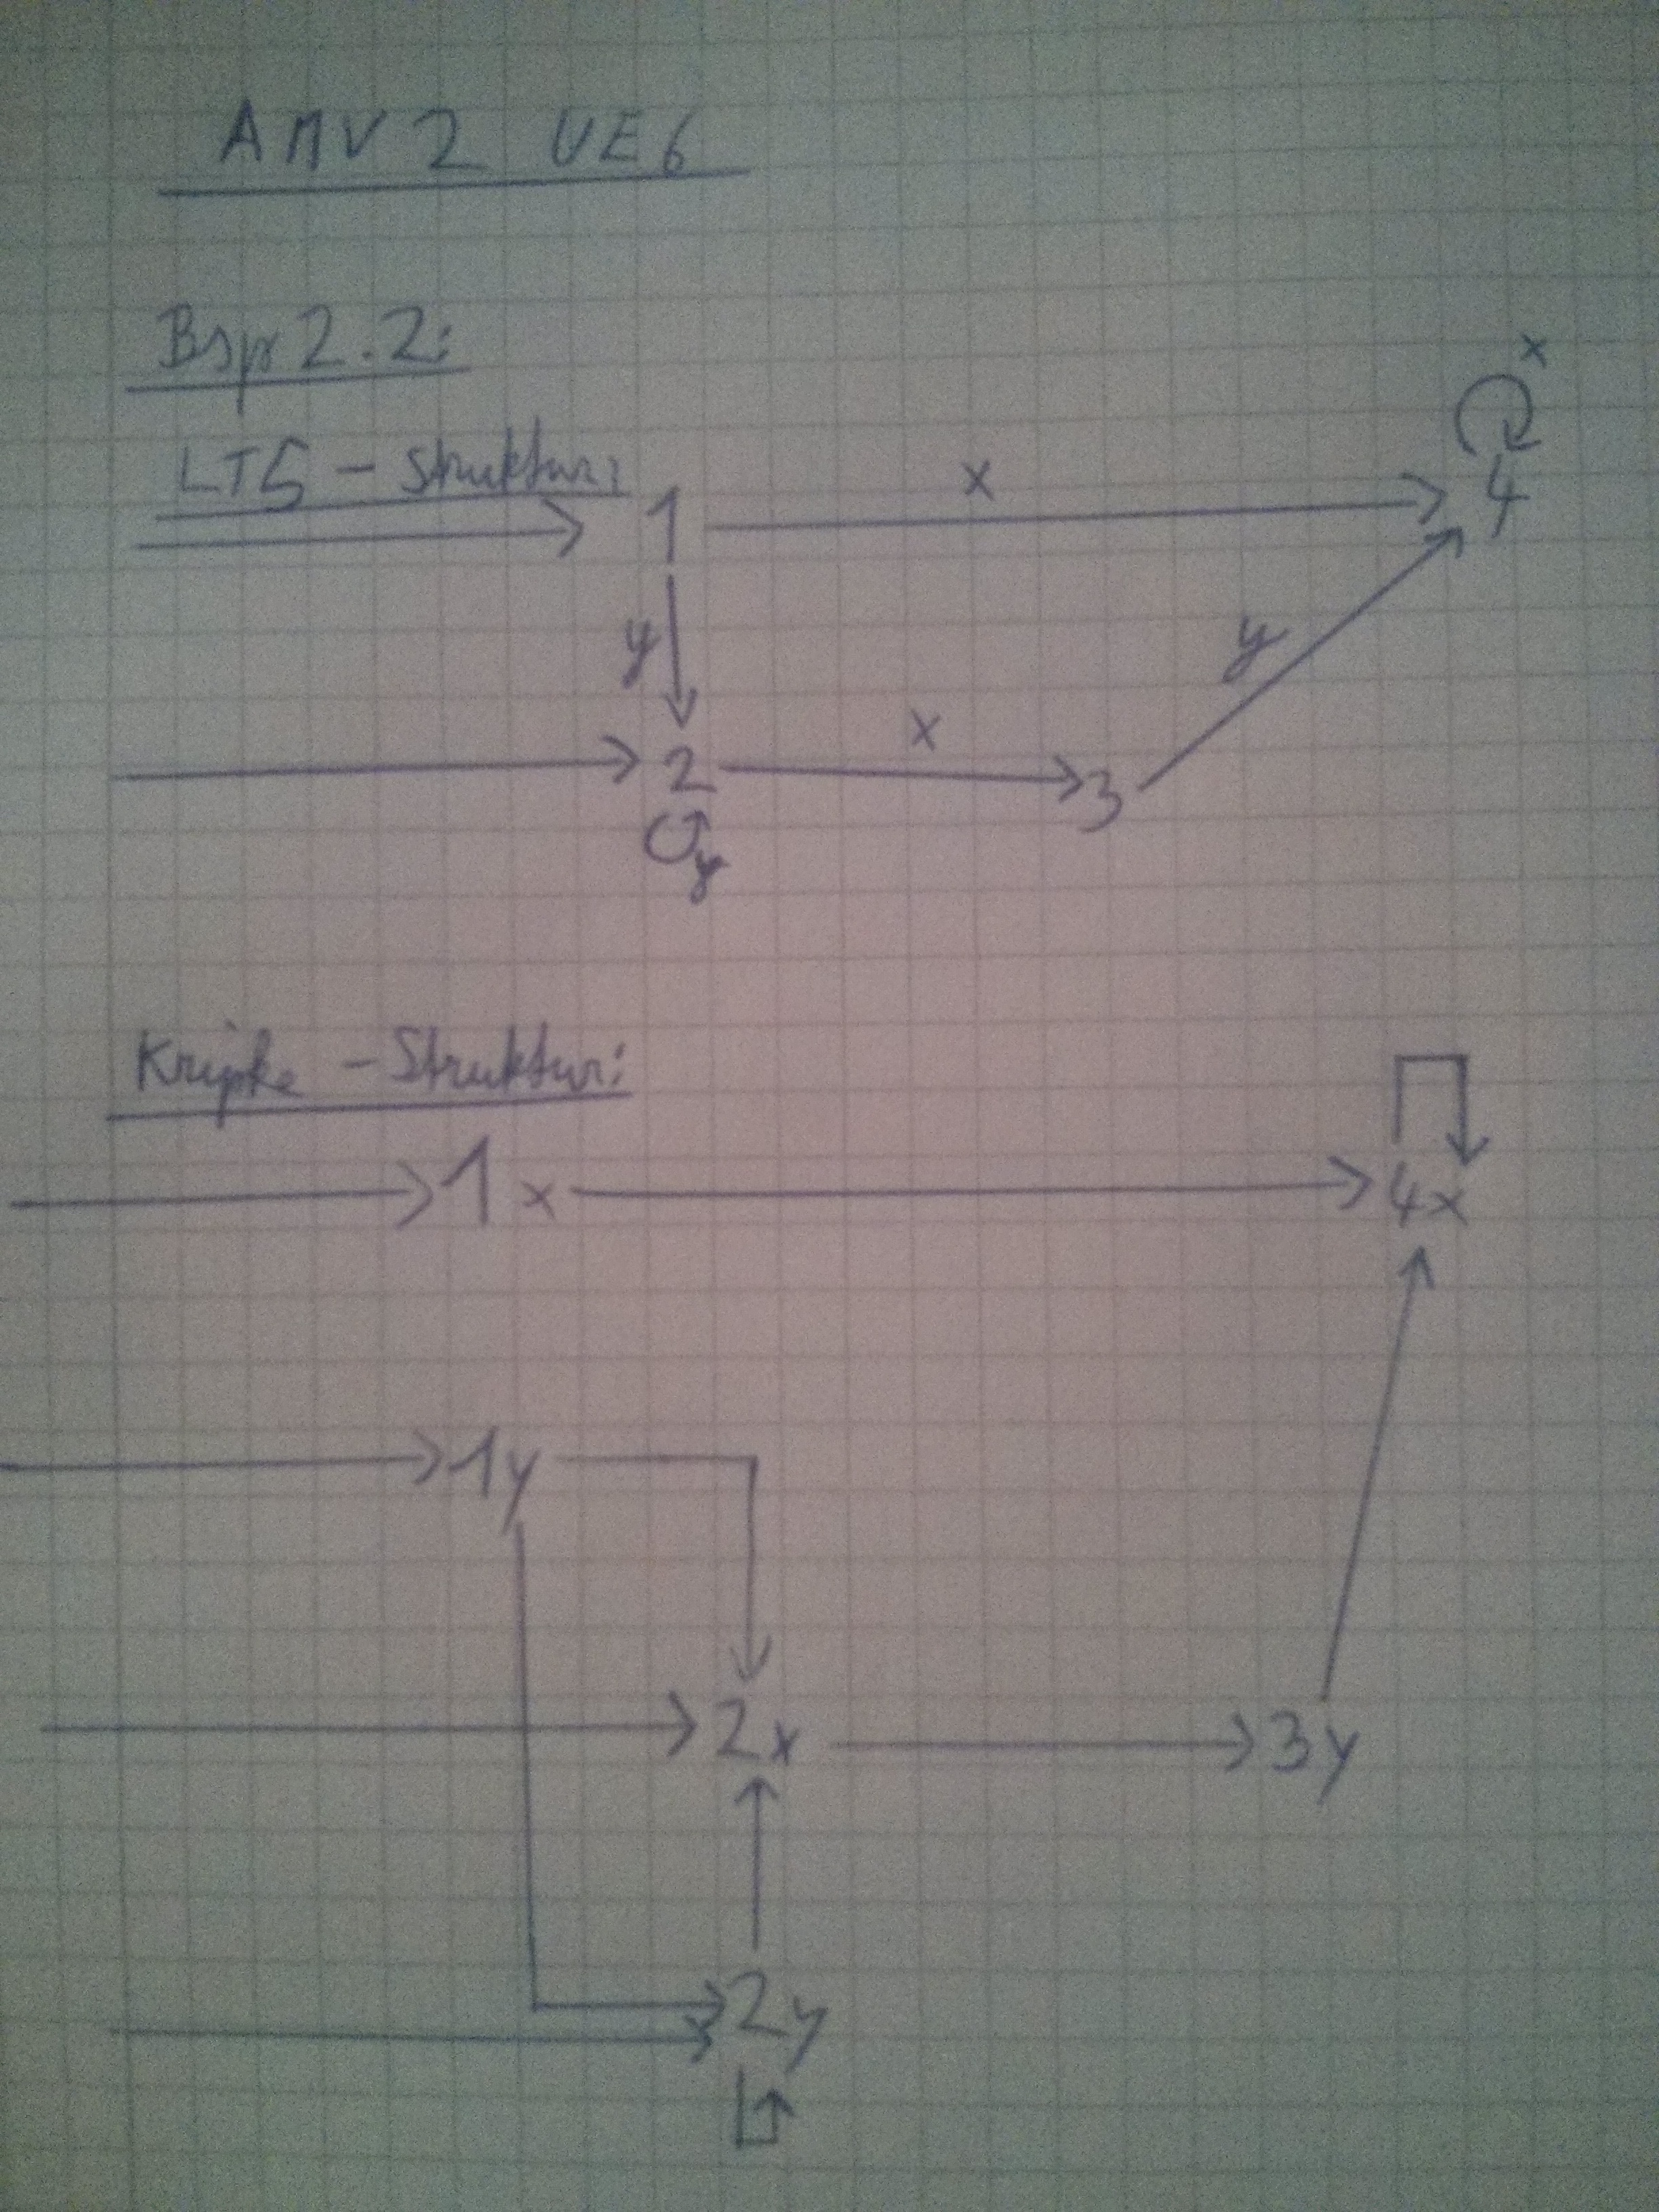
\includegraphics[width=\textwidth]{2.jpg}
\caption{Kripke}
\end{figure}

\end{document}
